\documentclass{beamer}
\usepackage{graphicx}
\usepackage{amssymb,amsfonts,amsmath}
\usepackage{tikz,tkz-euclide}
\usetikzlibrary{arrows.meta}
\usetikzlibrary{calc,patterns}
\usefonttheme[onlymath]{serif}
\usetheme{Berlin}
\title{Report 22th June}
\author{WU Zihan}
\subtitle{Detection of Ellipse}
\begin{document}
    \maketitle

    \begin{frame}
        \frametitle{Project Target}
    
        To detect ellipses in the images/videos.
        \begin{columns}
            \begin{column}{.5\linewidth}
                \begin{figure}
                    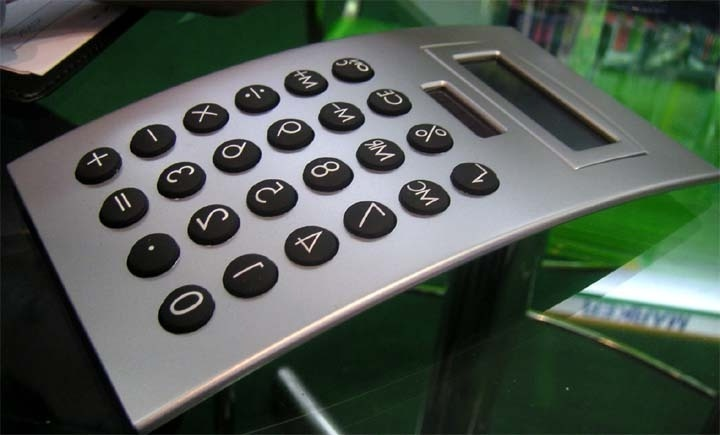
\includegraphics[width=0.8\linewidth]{pic/source.jpg}
                    \caption{Input}
                \end{figure}
            \end{column}
            \begin{column}{.5\linewidth}
                \begin{figure}
                    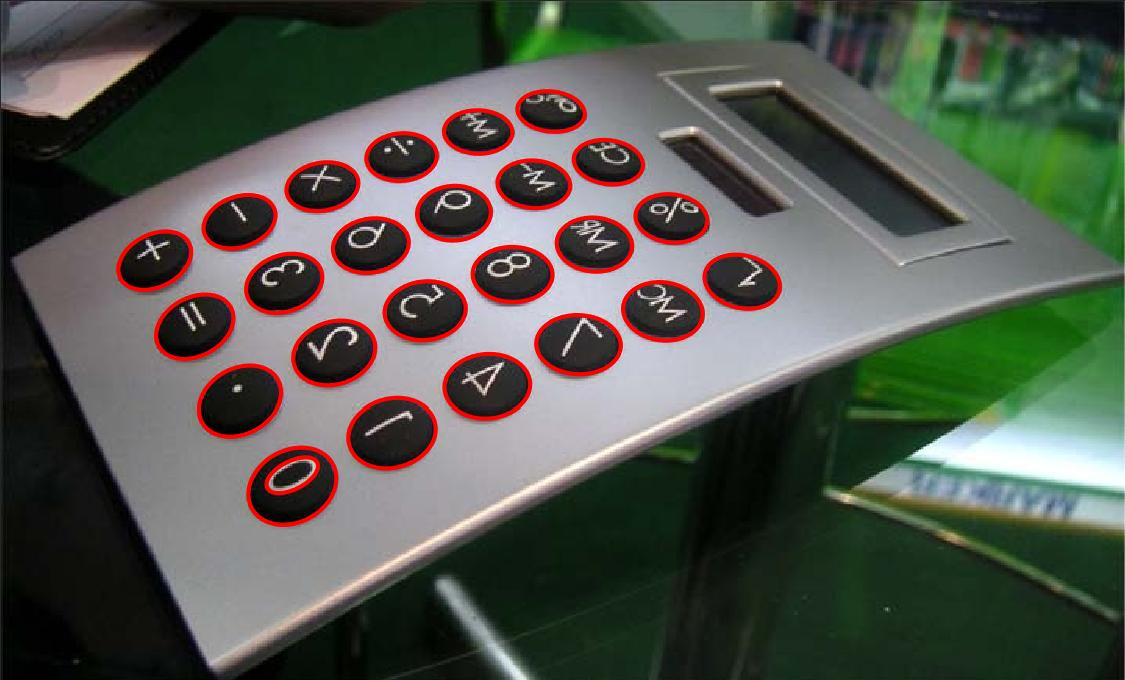
\includegraphics[width=0.8\linewidth]{pic/ideaoutput.jpg}
                    \caption{Output}
                \end{figure}
            \end{column}
        \end{columns}
    
    \end{frame}

    \begin{frame}
        \frametitle{Ellipse}

        To describe an ellispe we need 5 parameters:

        $$ Ax^2 + Bxy + Cy^2 + Dx + Ey + F = 0 , \text{where } B^2 - 4 AC < 0.$$

        Or in another way, we need the coordinates of ellipse's center ($x_0, y_0$), semi-major/semi-minor axes ($a,b$),
        and a rotation angle ($\varphi$).
        \begin{center}
            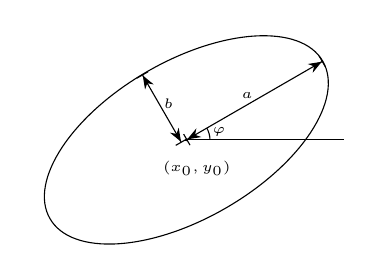
\begin{tikzpicture}
                \tikzstyle{every node}=[font=\tiny]
                \draw [rotate=30] (1,1) ellipse (2 and 1);
                \filldraw [rotate=30] (1,1) circle (.01);
                \draw [|{Stealth}-{Stealth}|,rotate=30,xshift =-2pt] (1,1)--(1,2);
                \draw [|{Stealth}-{Stealth}|,rotate=30] (1,1)--(3,1);
                \draw (0.5,1) node{$\left(x_0,y_0\right)$};
                \draw [xshift = 4pt,yshift = -2pt](0,1.9) node{$b$};
                \draw [xshift = 4pt,yshift = -2pt](1,2) node{$a$};
                \draw (0.366,1.366) -- (2.366,1.366 );
                \draw (0.666,1.366) arc (0:30:0.3);
                \draw (0.366,1.366) node[right,xshift = 6pt,yshift = 3pt]{$\varphi$};
                % \draw ({cos(75)} /{cos(45)} ,-1) -- ({cos(75)} /{cos(45)} ,1);
                % coordinate
                % \draw[->] (-3,0)--(3,0) node[right]{$x$};
                % \draw[->] (0,0)--(0,3) node[above]{$y$};
                % \draw[->,rotate = 30] (-3,0)--(3,0) node[right]{$x'$};
                % \draw[->,rotate = 30] (0,0)--(0,3) node[above]{$y'$};
                % \draw[->,rotate = 60] (-3,0)--(3,0) node[right]{$x''$};
                % \draw[->,rotate = 60] (0,0)--(0,3) node[above]{$y''$};
                % \draw [-,rotate=30] (1,1)--(-1,1);
            \end{tikzpicture}
        \end{center}
        

    \end{frame}

    \begin{frame}
        \frametitle{Two major ways}
        
        

        \begin{columns}
            \begin{column}{.5\linewidth}
                Hough Transform
                \begin{itemize}
                    \item Slow
                    \item Sacrifice accuracy for efficiency
                \end{itemize}
            \end{column}
            \begin{column}{.5\linewidth}
                Edge Following
                \begin{itemize}
                    \item Derived from Arc-support LS 
                    \item use greyscale image (gradient)
                    \item Greedy for efficiency
                \end{itemize}
            \end{column}
        \end{columns}
        
    \end{frame}

    \begin{frame}
        \frametitle{Methods}
    
        \begin{itemize}
            \item Detect the arc segements
            \item Form to acrs 
            \item Predict the 5 parameters for ellipses
            \item Co-cluster
            \item Validation
        \end{itemize}
    
    \end{frame}

\end{document}